\documentclass{article}



\usepackage{fullpage}
\usepackage{nopageno}
\usepackage{amsmath}
\usepackage{amsfonts}
\usepackage{graphicx}
\usepackage{framed}
\usepackage{xcolor}

\definecolor{dark_red}{rgb}{0.5,0.0,0.0}
\definecolor{dark_green}{rgb}{0.0,0.5,0.0}
\definecolor{dark_blue}{rgb}{0.0,0.0,0.5}

\newcommand{\dr}[1]{\textcolor{dark_red}{#1}}
\newcommand{\dg}[1]{\textcolor{dark_green}{#1}}
\newcommand{\db}[1]{\textcolor{dark_blue}{#1}}


\begin{document}


%%%%%%%%
\begin{framed}
\textbf{Problem 1:} Convert the following to radians, and express your answer as a multiple of \(\pi\) where the coefficient of \(\pi\) is in decimal form (no fractions) with 4 significant digits:
\begin{itemize}
\item \(67.00^\circ\)
\item \(-34.00^\circ\)
\item \(-100.0^\circ\)
\item \(255.0^\circ\)
\end{itemize} 
\dr{\textbf{Solution:} \\
\(67.00^\circ = \frac{\pi}{180^\circ}(67.00^\circ) \approx 0.3722\pi\) \\
\(-34.00^\circ = \frac{\pi}{180^\circ}(-34.00^\circ) \approx -0.1889\pi\) \\
\(-100.0^\circ = \frac{\pi}{180^\circ}(-100.0^\circ) \approx -0.5556\pi\) \\
\(255.0^\circ = \frac{\pi}{180^\circ}(255.0^\circ) \approx 1.417\pi\)
}
\end{framed}
%%%%%%%%
\begin{framed}
\textbf{Problem 2:} Convert the following to degrees, and express your answer in decimal form (no fractions) with 4 significant digits:
\begin{itemize}
\item \(0.2770\pi\)
\item \(0.6002\pi\)
\item \(-0.9900\pi\)
\item \(1.665\pi\)
\end{itemize}
\dr{\textbf{Solution:} \\
\(0.2770\pi = \frac{180^\circ}{\pi}(0.2770\pi) \approx 49.86^\circ\) \\
\(0.6002\pi = \frac{180^\circ}{\pi}(0.6002\pi) \approx 108.0^\circ\) \\
\(-0.9900\pi = \frac{180^\circ}{\pi}(-0.9900\pi) \approx -178.2^\circ\) \\
\(1.665\pi = \frac{180^\circ}{\pi}(1.665\pi) \approx 299.7^\circ\)
}
\end{framed}
%%%%%%%%
\pagebreak
\begin{framed}
\textbf{Problem 3:} ~~\\ ~~\\
\begin{tabular}{cc}
\parbox{0.4\textwidth}{
The image on the right shows the basic gear assembly for a bicycle. The foot pedals turn a front gear with a radius of \(r_F = 5\text{cm}\). The teeth of the front gear move a chain that turns the back gear with a radius of \(r_B = 2\text{cm}\). The back gear is then directly affixed to the back wheel with a radius of \(r_W = 40\text{cm}\). If the pedals are turning once every \(T = 1\text{s}\), compute:
\begin{itemize}
\item The angular speed \(\omega_F\) of the front gear.
\item The speed \(v_C\) of the chain. Hint: The chain's speed is the speed of the rims of both the front and back gear.
\item The angular speed \(\omega_B\) of the back gear.
\item The speed of the rim of the back wheel \(v_W\). This is the bike's speed. Hint: Since the back gear is directly affixed to the back wheel, the back gear and the back wheel share the same angular speed.
\end{itemize} 
} & \parbox{0.6\textwidth}{
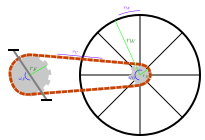
\includegraphics[width = 0.6\textwidth]{bicycle_gears}
}
\end{tabular}
\dr{\textbf{Solution:} \\
Using the period gives the angular speed of the front gear: 
\[\omega_F = \frac{2\pi}{T} = \frac{2\pi}{1.000 \times 10^0\text{s}} \approx 6.283 \times 10^0 \;\text{s}^{-1}\] %\frac{2\pi}{T}
Knowing the angular speed of the front gear, the speed of the chain, which is the speed of the front gear rim, is: 
\[v_C = r_F\omega_F = (5.000 \times 10^{-2} \;\text{m})(6.283 \times 10^0 \;\text{s}^{-1}) \approx 3.142 \times 10^{-1}\;\text{m/s}\] %\frac{2\pi r_F}{T}
Knowing the speed of the chain, which is the speed of the back gear rim, the angular speed of the back gear is:
\[\omega_B = \frac{v_C}{r_B} = \frac{3.142 \times 10^{-1} \;\text{m/s}}{2.000 \times 10^{-2} \;\text{m}} \approx 1.571 \times 10^1 \;\text{s}^{-1}\] %\frac{2\pi r_F}{T r_B}
Finally, knowing the angular speed of the back wheel, which is the angular speed of the back gear, the speed of the back wheel rim is:
\[v_W = r_W\omega_B = (4.000 \times 10^{-1} \;\text{m})(1.571 \times 10^1 \;\text{s}^{-1}) \approx 6.284 \times 10^0 \;\text{m/s}\] % \frac{2\pi r_F r_W}{T r_B} 
}
\end{framed}
%%%%%%%%
\pagebreak
\begin{framed}
\textbf{Problem 4:} ~~\\ ~~\\
\begin{tabular}{cc}
\parbox{0.4\textwidth}{
The image on the right, Bowser's underground castle is on the opposite side of a lava moat of unknown width \(w\). It is known that Bowser's castle has a height of \(y = 50\text{m}\). To figure out how to cross the moat, Mario uses surveying equipment to determine that the angle of elevation, from the ground on the edge of the moat, of the castle's summit is \(\theta = 14^\circ\). How wide is Bowser's moat?  
} & \parbox{0.6\textwidth}{
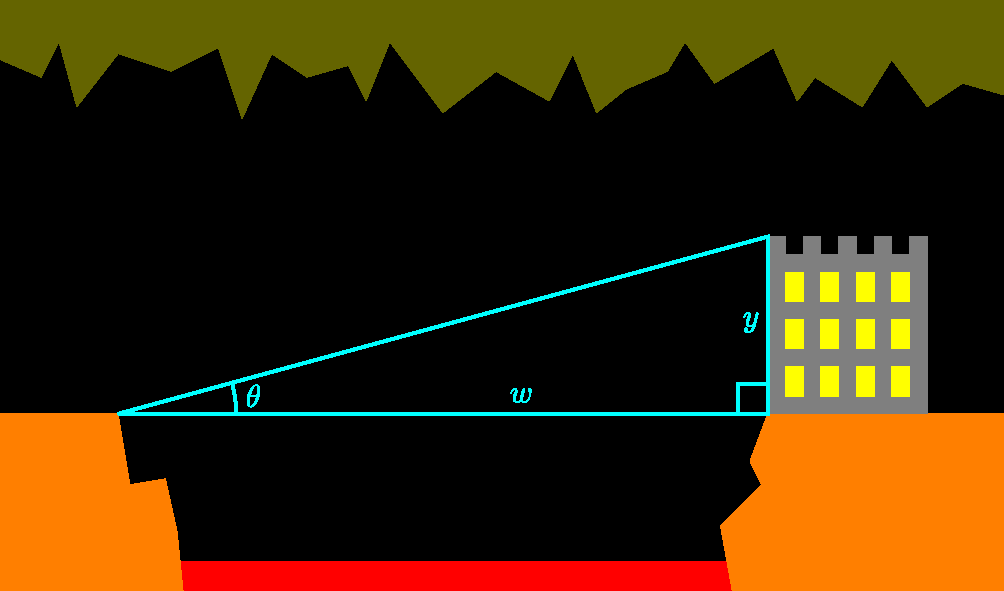
\includegraphics[width = 0.6\textwidth]{gorge_width}
}
\end{tabular}
\dr{\textbf{Soltuion:} \\ 
The opposite \(y = 5.000 \times 10^1 \;\text{m}\) is known, and the adjacent \(w\) is sought. Therefore the trigonometric ratio to be used is \(\cot\theta\):
\[w = y\cot\theta = (5.000 \times 10^1 \;\text{m})\cot(14^\circ) \approx 2.005 \times 10^2 \;\text{m} = 200.5\text{m}\]
}
\end{framed}



\end{document}







